\published{Geophysics, 82, DOI: 10.1190/geo2017-0554.1}

\title{EMD-seislet transform}
\renewcommand{\thefootnote}{\fnsymbol{footnote}}
\author{Yangkang Chen\footnotemark[1] and Sergey Fomel\footnotemark[2]}


\ms{GEO-2017-0554}

\address{
\footnotemark[1]Previously: 
John A. and Katherine G. Jackson School of Geosciences \\
The University of Texas at Austin\\
University Station\\
Box X, Austin, TX 78713-8924\\
Currently: 
National Center for Computational Sciences\\
Oak Ridge National Laboratory\\
One Bethel Valley Road\\
Oak Ridge, TN 37831-6008\\
chenyk2016@gmail.com\&cheny@ornl.gov\\
\footnotemark[2]
John A. and Katherine G. Jackson School of Geosciences \\
The University of Texas at Austin\\
University Station\\
Box X, Austin, TX 78713-8924\\
sergey.fomel@beg.utexas.edu 
}

\lefthead{Chen \& Fomel}
\righthead{EMD-seislet transform}
\maketitle

\begin{abstract}
The seislet transform uses a prediction operator which is connected to the local slope or frequency of seismic events. In this paper, we propose combining \new{the} 1D non-stationary seislet transform with empirical mode decomposition (EMD) in the $f-x$ domain. We use \new{the} EMD to decompose data into smoothly variable frequency components for the following 1D seislet transform. The resultant representation shows remarkable sparsity.  We introduce the detailed algorithm and use \old{one}\new{a} field example to demonstrate the application of the new seislet transform for sparsity-promoting seismic data processing.
\end{abstract}


\section{Introduction}
\new{The sparse}\old{Sparse} approximation aims at extracting the most important information of the given data by a linear combination of pre-specified atom signals with sparse linear coefficients. \old{Sparse approximation}\new{The} theory has been a rapidly evolving field in digital image analysis, since many state-of-the-art signal and image processing tasks have been successfully handled with the concept of sparsity, including image inpainting and restoration \cite[]{elad2005,shuwei20153,shuwei2016cs,amir2017}, image denoising \cite[]{mostafa2016geo,mostafa2017geo,amir2017geo}, data compression \cite[]{bryt2008}, blind source separation \cite[]{zib2001}, etc.

Over the past several decades, different types of sparse transforms have been explored for seismic \old{data processing }applications, and promising results have been reported \cite[]{yangkang20142}. 
\cite{fomel2010seislet} introduced a data-adaptive \old{sparsity promoting }transform, called the \emph{seislet} transform. Following the lifting scheme used in the construction of second-generation digital wavelets, the seislet transform utilizes the \old{spatial }predictability\old{ property} of \new{the} seismic data to construct the predictive operator. \cite{fomel2010seislet} used plane-wave construction (PWD) to aid the prediction process. Instead of using PWD, \cite{liuyang2010} used differential offset continuation (OC) to construct \new{a} seislet transform for pre-stack reflection data. \new{The} OC-seislet transform can obtain better sparsity for conflicting-dip pre-stack seismic data in that \new{the} OC seislet uses offset continuation instead of local slopes to connect different common offset gathers. %however, at the expense of much higher computational cost. 
In order to relieve the dependence of \new{the} seislet transform on local slope estimation, \cite{liuyang2015} proposed a velocity-dependent (VD) seislet transform based on conventional velocity analysis. The seislet transform has also found a recent application in simultaneous-source separation. Instead of using a single slope or frequency map to sparsify the seismic data, \cite{fomel2010seislet} proposed to apply several seislet transforms with smoothly variable slopes or frequencies, which are referred to as seislet frames.
 
In this paper, we propose to use empirical mode decomposition (EMD) \cite[]{huangemd} to create sparse transforms for representing seismic data.  The essence of \new{the} EMD is to stabilize a highly non-stationary signal by decomposing it into smoothly variable frequency components, which are called  intrinsic mode functions (IMF). We first transform the input seismic data from \new{the} $t-x$ domain to \new{the} $f-x$ domain, then apply \new{the} EMD to each frequency slice to decompose \new{the} input data into smooth\old{ly variable} frequency components. Next, \new{the} 1D non-stationary seislet transform is applied independently to each component. We evaluate the sparsity of the new representation (EMD-seislet transform) and apply it to noise attenuation of a seismic image.
\section{Method}
\subsection{Empirical mode decomposition}
The process of EMD has the following simple expression: 
\begin{equation}
\label{eq:emd}
s(t)=\sum_{n=1}^{N}c_n(t)+r(t),
\end{equation}
where $s(t)$ is the original non-stationary signal, $c_n(t)$ ($n=1,2,\cdots,N$) denotes each separated IMF, $N$ denotes the number of separated IMF, and $r(t)$ denotes the residual after EMD. The process of EMD is to gradually remove the stable oscillations embedded in the original signal to arrive at a monotonic and smooth residual or trend at last. A special property of \new{the} EMD is that the IMFs represent different oscillations embedded in the data, where the oscillating frequency for each sub-signal $c_n(t)$ decreases with IMF order increasing \cite[]{huangemd}. 

\subsection{1D seislet transform}
The seislet transform can be constructed by multi-scale prediction of the odd components $\mathbf{o}$ from the even components $\mathbf{e}$:
\begin{align}
\label{eq:r}
\mathbf{r}&=\mathbf{o}-\mathbf{P}(\mathbf{e}), \\
\label{eq:e}
\mathbf{c}&=\mathbf{e}+\mathbf{U}(\mathbf{r}).
\end{align}
\new{In the above equations,} $\mathbf{P}$ denotes the prediction operator and $\mathbf{U}$ denotes the updating operator at a particular scale. \new{$\mathbf{r}$ denotes the difference vector and $\mathbf{c}$ denotes the updated even component.} The inverse seislet transform follows the inverse process of equations \ref{eq:r} and \ref{eq:e} continuing from large to small scale. The difference between \new{the} 1D seislet transform and \new{the} 1D wavelet transform is whether the prediction is modulated by an appropriate frequency. In the simplest case of Haar transform, the Z-transform domain prediction filter for the Haar wavelet transform is 
\begin{equation}
\label{eq:haar}
P(Z)=Z,
\end{equation}
and the Z-transform domain Haar prediction filter for wavelet transform is 
\begin{equation}
\label{eq:haaru}
U(Z)=Z/2.
\end{equation}

However, for \new{the} seislet transform,
\begin{align}
\label{eq:haarseis}
P(Z)&=Z/Z_0, \\
\label{eq:haarseisu}
U(Z)&=1/2(Z/Z_0).
\end{align}
where $Z_0=e^{i\omega_0\Delta t}$. The prediction filter \new{in equation} \ref{eq:haarseis} can perfectly characterize\old{s} a sinusoid with $\omega_0$ \old{circular}\new{angular} frequency sampled on a $\Delta t$ grid.
Analogously, the prediction filter for biorthogonal 2/2 transform can be expressed as:
\begin{equation}
\label{eq:linearseis0}
P(Z)=1/2(Z/Z_0+Z_0/Z),
\end{equation}
and its corresponding updating operator is
\begin{equation}
\label{eq:uplinearseis0}
U(Z)=1/4(Z/Z_0+Z_0/Z).
\end{equation}

\subsection{1D non-stationary seislet transform}
%Let us take the linear prediction filter \ref{eq:linearseis} as an example.
When a 1D signal has a constant \old{circular}\new{angular} frequency, the prediction filter \new{in equation} \ref{eq:haarseis} can characterize a sinusoidal signal. When the 1D signal contains a sinusoid with a variable frequency, or in other words, is non-stationary, we can replace $Z_0$ with $Z_t$,  $Z_t=e^{i\omega(t)\Delta t}$ denotes the frequency modulation at time $t$. Let us modify equation \ref{eq:linearseis0} to the following form\new{:}
\begin{equation}
\label{eq:linearseis}
P_t(Z) = 1/2(Z/Z_t + Z_t/Z),
\end{equation}
in order to best characterize the non-stationary signal. $P_t(Z)$ denotes the prediction filter at time $t$.\old{, and $Z_t=e^{i\omega(t)\Delta t}$ denotes the frequency modulation at time $t$.} In the physical domain, the linear prediction and updating operators can be expressed as:
\begin{align}
\label{eq:linearseis-phy}
P_t(e)&=(S_t^{(+)}(e_{t-1}) + S_t^{(-)}(e_t))/2,\\
\label{eq:linearseisu-phy}
U_t(r)&=(S_t^{(+)}(r_{t-1}) + S_t^{(-)}(r_t))/4,
\end{align}
where $S_t^{(+)}$ and $S_t^{(-)}$ are operators that predict an element from its left and right neighbors by modulating each element according to their local frequency $\omega(t)$.

Figure \ref{fig:non-comp2} shows a comparison between \new{the} wavelet transform and \new{the} 1D stationary and non-stationary seislet transforms in compressing a 1D signal with smooth\old{ly variable} frequency components. The frequency ranges from 250 to 186 Hz. Both the wavelet transform and stationary seislet transform fail to compress the signal well while the non-stationary seislet transform obtains a perfectly sparse representation.



\subsection{Estimating local frequency by complex non-stationary autoregression}
According to the autoregressive spectral analysis theory \cite[]{marple}, a complex time series that has a constant frequency component is predictable by a two-point prediction-error filter $(1,-e^{i\omega_0\Delta t})$. Suppose a complex time series is $d(t)$. In Z-transform notation, the two-point prediction-error filter can be expressed as:
\begin{equation}
\label{eq:twopre}
F(Z)=1-Z/Z_0.
\end{equation} 
We assume that a 1D time series \old{have}\new{has} a smooth\old{ly variable} frequency component, then the 1D time series can be locally predicted using different local two-point prediction-error filters $(1,-e^{i\omega(t)\Delta t})$:
\begin{equation}
\label{eq:localpre}
d(t)=e^{i\omega(t)\Delta t}d(t-\Delta t).
\end{equation}

In order to estimate $\omega(t)$ using equation \ref{eq:localpre}, we need to first minimize the least-squares misfit of the true and predicted time series with a local-smoothness constraint:
\begin{equation}
\label{eq:mini}
\min_{\mathbf{a}} \parallel \mathbf{d} - \mathbf{D} \mathbf{a} \parallel_2^2 + \mathbf{R}(\mathbf{a}),
\end{equation}
where $\mathbf{d}$ and $\mathbf{a}$ are \old{vector}\new{vectors} composed of the entries $d(t)$ and $a(t)$, respectively, and $a(t)=e^{i\omega(t)\Delta t}$. $\mathbf{D}$ is a diagonal matrix composed of the entries $d(t-\Delta t)$. $\mathbf{R}$ denotes the local-smoothness constraint. Equation \ref{eq:mini} can be solved using shaping regularization:
\begin{equation}
\hat{\mathbf{a}} = [\lambda^2\mathbf{I}+\mathcal{T}(\mathbf{D}^T\mathbf{D}-\lambda^2\mathbf{I})]^{-1}\mathcal{T}\mathbf{D}^T\mathbf{d},
\end{equation}
where $\mathcal{T}$ is a triangle smoothing operator and $\lambda$ is a scaling parameter that controls the physical dimensionality and enables fast convergence. $\lambda$ can be chosen as the least-squares norm of $\mathbf{D}$. After the filter coefficient $a(t)$ is obtained, we can straightforwardly calculate the local \old{circular}\new{angular} frequency $\omega(t)$ by
\begin{equation}
\label{eq:circ}
\omega(t) = Re\left[\frac{\mbox{arg}(a(t))}{\Delta t}\right].
\end{equation}

\subsection{Preparing locally stationary frequency slice by EMD}
The aforementioned 1D non-stationary seislet transform adapts to 1D signals that have smoothly variable  frequency components since its compression performance is controlled by the predicting and updating procedures between the series elements according to a locally smooth modulation frequency. Correspondingly, when calculating the local frequency, we also assume the 1D signal to have smoothly variable frequency components.  

We call the combined FFT-EMD-seislet workflow the \emph{EMD-seislet} transform. Figures \ref{fig:demo,demo-fz,demo,demo-fs-3} and \ref{fig:demo-f1z-0,demo-f1z-seis-0,demo-dip1-0,demo-f2z-0,demo-f2z-seis-0,demo-dip2-0,demo-f3z-0,demo-f3z-seis-0,demo-dip3-0} provide a detailed demonstration of the procedures involved in the EMD-seislet transform construction. Figure \ref{fig:demo} shows a synthetic data with hyperbolic events. Figure \ref{fig:demo-fz} shows the $f-x$ spectrum of the synthetic data. \new{Figure \ref{fig:demo-fs-3} shows a demonstration for preparing smoothly variable frequency components for each frequency slice using \new{the} EMD in the $f-x$ domain.} We can observe that each frequency slice in the $f-x$ domain is highly non-stationary. After EMD decomposition, the three decomposed $f-x$ domain components are shown in the left column of Figure \ref{fig:demo-f1z-0,demo-f1z-seis-0,demo-dip1-0,demo-f2z-0,demo-f2z-seis-0,demo-dip2-0,demo-f3z-0,demo-f3z-seis-0,demo-dip3-0}. Each component now has smoothly non-stationary frequency slices. After 1D non-stationary seislet transforms, the three $f-x$ domain components become highly compressed. The middle column in Figure \ref{fig:demo-f1z-0,demo-f1z-seis-0,demo-dip1-0,demo-f2z-0,demo-f2z-seis-0,demo-dip2-0,demo-f3z-0,demo-f3z-seis-0,demo-dip3-0} shows the compressed $f-x$ domain using the 1D non-stationary seislet transform. \new{The scale of the compressed coefficients is indicated by the horizontal axis.} The right column in Figure \ref{fig:demo-f1z-0,demo-f1z-seis-0,demo-dip1-0,demo-f2z-0,demo-f2z-seis-0,demo-dip2-0,demo-f3z-0,demo-f3z-seis-0,demo-dip3-0} shows the reconstructed $t-x$ domain data from the decomposed and compressed components in the middle column. The three decomposed components correspond to different parts of the input signal.% three different slopes. % The EMD-seislet transform domain appears sparse.

In order to compare the sparsity in compressing seismic data, we plot the reconstruction error curves with respect to the number of selected largest coefficients. The reconstruction error is defined as $E=\parallel\mathbf{d}-\mathbf{Am}_N\parallel_2^2$, where $\mathbf{m}_N$ denotes the largest $N$ coefficients in the transform domain. The faster the curve decays, the sparser the corresponding transform domain will be. As shown in Figure \ref{fig:sparse}, the EMD-seislet appears to be the sparsest compared with the PWD-seislet transform, wavelet transform, and Fourier transform.

\section{Application \old{to}\new{of} noise attenuation \old{of}\new{to} real data}
We use a \old{field}\new{real} data example shown in Figure \ref{fig:real-0} to demonstrate the performance of the proposed EMD-seislet in attenuating random noise. Figure \ref{fig:real-eseist-0} shows the denoised result by thresholding in the EMD-seislet transform domain. Figure \ref{fig:real-eseist-dif-g} shows the removed noise section using EMD-seislet thresholding. 2\% of EMD-seislet coefficients were retained. Despite the complicated structures of the seismic image, the proposed approach obtains a successful denoising performance. \new{Figure \ref{fig:real-seist-0} shows the denoised result using the traditional seislet thresholding method. Figure \ref{fig:real-fx-0} shows the denoised result using the FX Decon method. Figures \ref{fig:real-seist-dif-g} and \ref{fig:real-fx-dif-g} show the removed noise corresponding to the seislet thresholding method and the FX Decon method, respectively. Figures \ref{fig:real-z}, \ref{fig:real-eseist-z}, \ref{fig:real-seist-z}, and \ref{fig:real-fx-z} show the enlarged sections (corresponding to the frame boxes in Figure \ref{fig:real-eseist-0,real-eseist-dif-g,real-seist-0,real-seist-dif-g,real-fx-0,real-fx-dif-g}).} From the comparison in Figure \ref{fig:real-eseist-0,real-eseist-dif-g,real-seist-0,real-seist-dif-g,real-fx-0,real-fx-dif-g},  
the proposed approach obtains the best result, while \new{the} seislet thresholding is over-smoothing\new{,} and \new{the} FX Decon harms some of the signal energy. \new{The over-smoothing effect of the seislet thresholding method may be due to the over-smooth local slope calculated using the PWD algorithm. The signal-leakage problem of the FX Decon method has been widely studied in the literature, e.g., in \cite{yangkang20141}.} \new{The EMD-seislet domains before and after applying the thresholding operator are plotted in Figures \ref{fig:real-femdr-seis0-3d} and \ref{fig:real-femdr-seis-thr-3d}, respectively. It is clear that the thresholding removes most low-amplitude coefficients in the sparse EMD-seislet domain.}


\section{Conclusion}
We have proposed a novel approach for sparsifing seismic data: EMD-seislet transform. The approach relies on the ability of empirical mode decomposition (EMD) in the $f-x$ domain to provide smoothly non-stationary data, which we use in the following 1D non-stationary seislet transform. When applied to seismic data with multiple conflicting slopes, EMD-seislet is remarkably sparse. A \old{field}\new{real} data example shows an excellent performance of \new{the} EMD-seislet transform in attenuating random noise. \new{However, the large computational cost required by the EMD algorithm requires a careful design of the parallel computing framework in the future research. }


\new{
\section{Acknowledgments}
We appreciate the comments from three anonymous reviewers that greatly improved the manuscript.
}


\inputdir{nonseis}

\plot{non-comp2}{width=0.8\textwidth}{Demonstration of 1D non-stationary seislet transform for \new{a} non-stationary signal. \old{Upper}\new{From the top to the bottom: non-stationary chirp signal (frequency ranges from 250 to 186 Hz), compressed data using \new{the} 1D wavelet transform, compressed data using \new{the} 1D stationary seislet transform with the frequency of 250 Hz, and compressed data using \new{the} 1D non-stationary seislet transform.}}


\begin{figure}[htb!]
  \centering
  \subfloat[]{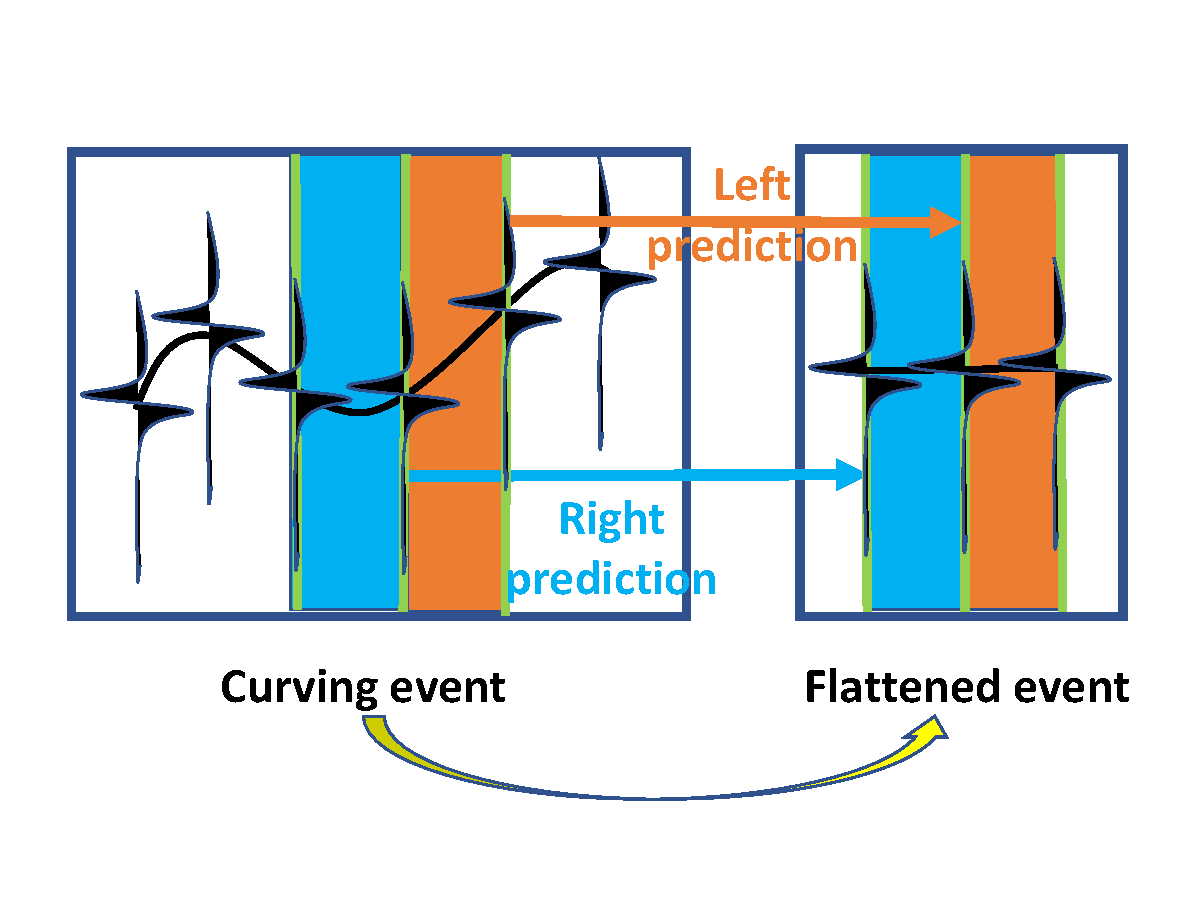
\includegraphics[width=0.3\textwidth]{demo2/Fig/demo}
    \label{fig:demo}}
  \subfloat[]{\includegraphics[width=0.3\textwidth]{demo2/Fig/demo-fz}
    \label{fig:demo-fz}}\\
  \subfloat[]{\includegraphics[width=0.7\textwidth]{demo2/Fig/demo-fs-3}
    \label{fig:demo-fs-3}}
   \caption{(a) Synthetic example with hyperbolic events. (b) $f-x$ spectrum of (a). (c) Demonstration of preparing the smoothly variable frequency components by \new{the} EMD for the 15 Hz slice of the synthetic data in Figure \ref{fig:demo}.}
   \label{fig:demo,demo-fz,demo,demo-fs-3}
\end{figure}

\inputdir{demo4}
\multiplot{9}{demo-f1z-0,demo-f1z-seis-0,demo-dip1-0,demo-f2z-0,demo-f2z-seis-0,demo-dip2-0,demo-f3z-0,demo-f3z-seis-0,demo-dip3-0}{width=0.24\textwidth}{A demonstration of the EMD-seislet transform. The left column shows the decomposed $f-x$ domain spectrum using the EMD. The middle column shows the compressed $f-x$ domain using 1D non-stationary seislet transform. The right column shows the reconstructed $t-x$ domain data corresponding to different components.}

\inputdir{sparse}
\plot{sparse}{width=0.8\columnwidth}{Sparsity comparison. $E=\parallel\mathbf{d}-\mathbf{Am}_N\parallel_2^2$ denotes the reconstruction error with the largest $N$ coefficients in the transform domain.}


\begin{figure}[htb!]
  \centering
  \subfloat[]{\includegraphics[width=0.3\textwidth]{field/Fig/real-0}
    \label{fig:real-0}}
  \subfloat[]{\includegraphics[width=0.2\textwidth]{field/Fig/real-z}
    \label{fig:real-z}}\\
  \subfloat[]{\includegraphics[width=0.3\textwidth]{field/Fig/real-eseist-0}
    \label{fig:real-eseist-0}}
  \subfloat[]{\includegraphics[width=0.3\textwidth]{field/Fig/real-eseist-dif-g}
    \label{fig:real-eseist-dif-g}} 
  \subfloat[]{\includegraphics[width=0.2\textwidth]{field/Fig/real-eseist-z}
    \label{fig:real-eseist-z}}\\
  \subfloat[]{\includegraphics[width=0.3\textwidth]{field/Fig/real-seist-0}
    \label{fig:real-seist-0}}
  \subfloat[]{\includegraphics[width=0.3\textwidth]{field/Fig/real-seist-dif-g}
    \label{fig:real-seist-dif-g}} 
  \subfloat[]{\includegraphics[width=0.2\textwidth]{field/Fig/real-seist-z}
    \label{fig:real-seist-z}}\\
  \subfloat[]{\includegraphics[width=0.3\textwidth]{field/Fig/real-fx-0}
    \label{fig:real-fx-0}}
  \subfloat[]{\includegraphics[width=0.3\textwidth]{field/Fig/real-fx-dif-g}
    \label{fig:real-fx-dif-g}}
  \subfloat[]{\includegraphics[width=0.2\textwidth]{field/Fig/real-fx-z}
    \label{fig:real-fx-z}}
   \caption{Denoising test. (a) Real seismic data. (c) Denoised data using EMD-seislet domain thresholding. (d) Noise section \old{corresponds}\new{corresponding}  to (c).  (f) Denoised data using seislet domain thresholding. (g) Noise section \old{corresponds}\new{corresponding} to (f). (i) Denoised data using FX Decon. (j) Noise section \old{corresponds}\new{corresponding} to (i). (b),(e),(h) and (k): Zoomed sections for the frame boxes \new{in (a), (c), (f), and (i), respectively}.}
   \label{fig:real-eseist-0,real-eseist-dif-g,real-seist-0,real-seist-dif-g,real-fx-0,real-fx-dif-g}
\end{figure}
\inputdir{field}
\multiplot{2}{real-femdr-seis0-3d,real-femdr-seis-thr-3d}{width=0.45\textwidth}{\new{(a) EMD-seislet domain before thresholding. (b) EMD-seislet domain after thresholding.}}

\bibliographystyle{seg}
\bibliography{eseis}

\newpage
\listoffigures

